%*********************************************************************
\chapter{Theoretical development}
\label{ch:theory}

Section~\ref{sec:multivariable-control} established that the usual route to a PID controller for an enclosure like this one is to write a balance equation for the chamber, transform it, and design the controller against the resulting transfer function \citep{matamoros_temperature_2020}. This chapter does that for temperature and CO\textsubscript{2}, then designs and simulates a PI controller for each loop.

Each model is lumped: the chamber air, the glass, the plate and the sample are treated as single nodes at uniform temperature, and each model gives a first-order transfer function between one actuator and one measurement. Spatial gradients, air movement inside the chamber and the optical properties of the lid are not modelled. Humidity is not modelled as a loop; it enters only as the constraint that the glass must stay warmer than the chamber, which is what keeps condensation off the optical path. The models are built before the hardware exists, so that the controllers can be tuned in simulation and so that it is clear which quantities have to be measured once the incubator is built. All parameter values are estimates based on geometry, material properties and datasheet figures, and are revisited in the chapters that follow.

\section{Thermal Models}
\label{sec:temperature-model}

\subsection{Approach}
\label{subsec:modelling-approach}

The chamber is modelled as a lumped RC thermal network. Each body that stores heat becomes a node with a single temperature and a thermal capacitance, the heat required to raise that temperature by one kelvin. Each path along which heat can travel becomes a thermal resistance, setting how much heat flows for a given temperature difference. The model is one differential equation per node, stating that the heat stored in that body changes at the rate of heat in minus heat out. The network is described as RC because these relationships are the same as those in an electrical circuit: Fourier's law of conduction and Newton's law of cooling both give a heat flow equal to a temperature difference divided by a resistance, which is the form of Ohm's law, and thermal capacitance plays the part of electrical capacitance \citep{incropera_fundamentals_2007}.

Representing a body by a single temperature assumes it is isothermal, which holds when conduction through the body is fast compared with heat loss from its surface, the ratio the Biot number expresses \citep{incropera_fundamentals_2007}. The glass is thin and satisfies the condition. The chamber air is a small volume and is assumed to be well mixed, and two sensors at different positions test that assumption once the chamber is built. The model is an approximation: the air will not be perfectly mixed, the walls will be warmer close to the heaters, and the sample will lie somewhere between the air and the plate temperature. What matters for controller design is that the dominant time constant and the steady-state gain are close to the real values, since a PI controller is tuned from those.

The model uses the components selected in Chapter~\ref{ch:design}, which were ordered early because of their lead times and chosen against the requirements in Section~\ref{sec:requirements} rather than against the model. It assumes 12\,W polyimide film heaters on the chamber walls, an ITO glass heater of 150 $\times$ 112 $\times$ 1.1\,mm as the lid, a 96-well plate of 127.76 $\times$ 85.48\,mm with a 1\,mm well base, and temperature sensors in the chamber, on the glass and in ambient air. The mechanical design was not finalised at the time, so the internal chamber is taken as 213 $\times$ 155 $\times$ 30\,mm.

\subsection{Chamber model}
\label{subsec:chamber-balance}

\begin{figure}[htbp]
\centering
\begin{circuitikz}[american, scale=0.8, transform shape]
  \ctikzset{bipoles/length=1cm}
  \draw (-3.4,0) -- (5.4,0);
  \node[right] at (5.4,0) {$T_a$};
  \draw (0.8,0) node[ground]{};
  \draw (-3,0) to[I, l=$\mu_h P_h$] (-3,4);
  \draw (-3,4) -- (0,4);
  \draw (-1.3,4) to[C, l=$C_c$] (-1.3,0);
  \node[circle,fill,inner sep=1.6pt] at (0,4) {};
  \node[below left] at (0,4) {$T_c$};
  \draw (0,4) to[R, l=$R_{cg}$] (0,6.6);
  \node[circle,draw,inner sep=2pt] at (0,6.6) {};
  \node[above] at (0,6.8) {$T_g$};
  \draw (0,4) -- (5,4);
  \draw (2.4,4) to[R, l=$R_{ca}$] (2.4,0);
  \draw (5,4) to[R, l=$R_{cp}$] (5,0);
\end{circuitikz}
\caption[Chamber RC network]{\textbf{Chamber as an RC network.} Ambient is the reference. The wall heaters are a current source into the chamber node and heat leaves along two parallel paths, through the walls and through the multiwell plate in the base.}
\label{fig:chamber-rc}
\end{figure}

Figure~\ref{fig:chamber-rc} shows the chamber as an RC network with ambient as the reference. Heat enters the chamber air from the film heaters and from the ITO glass above, which is held warmer than the chamber to keep condensation off the optical path \citep{noauthor_stage_nodate}. Heat leaves along two parallel paths, through the walls and through the multiwell plate in the base. The energy balance is

\begin{equation}
C_c \frac{dT_c}{dt} = \mu_h P_h + \frac{T_g - T_c}{R_{cg}} - \frac{T_c - T_a}{R_{ca}} - \frac{T_c - T_a}{R_{cp}}
\label{eq:chamber-balance}
\end{equation}

where $T_c$, $T_g$ and $T_a$ are the chamber air, glass and ambient temperatures, $C_c$ is the heat stored by the chamber air together with the printed wall around it, $P_h$ is the film heater power at full duty and $\mu_h$ is the duty cycle between 0 and 1. The three thermal resistances are chamber to glass ($R_{cg}$), chamber to ambient through the walls ($R_{ca}$) and chamber to ambient through the plate ($R_{cp}$). The heaters are switched by pulse-width modulation (PWM), so $\mu_h P_h$ is the average power over a switching period, which holds because the switching period is far shorter than the thermal time constants. The glass appears as an exchange term rather than a power input, since it is a node in the network and not a source, so the term adds heat whenever the glass is above the chamber temperature.

Grouping the $T_c$ terms in Equation~\ref{eq:chamber-balance} and taking the Laplace transform gives

\begin{equation}
T_c(s) = \frac{\mu_h(s) P_h + \dfrac{T_g(s)}{R_{cg}} + T_a(s) \left[ \dfrac{1}{R_{ca}} + \dfrac{1}{R_{cp}} \right]}{C_c s + \dfrac{1}{R_{cg}} + \dfrac{1}{R_{ca}} + \dfrac{1}{R_{cp}}}
\;=\;
\frac{K_h\,\mu_h(s) + K_g\,T_g(s) + K_a\,T_a(s)}{\tau s + 1},
\label{eq:chamber-tf}
\end{equation}

where $R_{tot}$ is the three resistances in parallel, $K_h = P_h R_{tot}$, $K_g = R_{tot}/R_{cg}$, $K_a = R_{tot}(1/R_{ca} + 1/R_{cp})$ and $\tau = C_c R_{tot}$. This is a first order model with one control input, the heater duty cycle, and two disturbances: the glass temperature, which has its own control loop, and the ambient temperature, which is measured but not controlled.

Evaluating the resistances and capacitances from the geometry and material properties gives a chamber time constant of about 10 minutes and a steady-state gain of 128\,K per unit duty. The parameter values and the reasoning behind the ones that are not simply geometry are given in Appendix~\ref{app:model-parameters} (Table~\ref{tab:thermal-params}), with the resistances worked through in Equations~\ref{eq:rca} to~\ref{eq:rcp}. Substituting into Equation~\ref{eq:chamber-tf} and normalising,

\begin{equation}
T_c(s) = \frac{36 \mu_h(s) + \dfrac{T_g(s)}{11.9} + 0.197\,T_a(s)}{167s + 0.281} = \frac{128 \mu_h(s) + 0.299\,T_g(s) + 0.701\,T_a(s)}{594s + 1}.
\label{eq:chamber-tf-final}
\end{equation}

The chamber time constant is about 594\,s, or 10\,min. The gain of 128\,K per unit duty means the heaters could raise the chamber far above any useful setpoint, so only a small duty cycle is needed to hold 37\,\textdegree{}C. With the glass at 39\,\textdegree{}C and the room at 19\,\textdegree{}C, Equation~\ref{eq:chamber-tf-final} predicts a steady duty of about 9\%, which is a concrete prediction to test against the built chamber. With no active cooling, the large gain also makes overshoot the main risk in the controller design.

\subsection{Glass model}
\label{subsec:glass-model}

The glass is modelled the same way, as a single node with its own heater. Heat enters from the ITO coating and leaves along two paths, down to the chamber air and up to the room. The glass also rests on the printed wall around its edges, which adds a conduction path to the room in parallel with $R_{ga}$. This is neglected here because the contact width is not yet fixed, although it would increase the power needed to hold the glass temperature and leave the edges cooler than the centre; the step test on the built glass includes this path. The balance and its transfer function take the same form as the chamber,

\begin{align}
C_g \frac{dT_g}{dt} &= \mu_g P_g + \frac{T_c - T_g}{R_{cg}} - \frac{T_g - T_a}{R_{ga}}, \label{eq:glass-balance} \\[4pt]
T_g(s) &= \frac{\mu_g(s) P_g + \dfrac{T_c(s)}{R_{cg}} + \dfrac{T_a(s)}{R_{ga}}}{C_g s + \dfrac{1}{R_{cg}} + \dfrac{1}{R_{ga}}}
\;=\;
\frac{K_{gh}\,\mu_g(s) + K_{gc}\,T_c(s) + K_{ga}\,T_a(s)}{\tau_g s + 1},
\label{eq:glass-tf}
\end{align}

where $R_{tot,g}$ is the two resistances in parallel, $K_{gh} = P_g R_{tot,g}$, $K_{gc} = R_{tot,g}/R_{cg}$, $K_{ga} = R_{tot,g}/R_{ga}$ and $\tau_g = C_g R_{tot,g}$, with the chamber temperature now the disturbance from the other loop. Equations~\ref{eq:glass-balance} and~\ref{eq:glass-tf} mirror Equations~\ref{eq:chamber-balance} and~\ref{eq:chamber-tf}, and the parameter values are in Table~\ref{tab:glass-params}.

The heater power needs an estimate because the ITO coating is specified by sheet resistance, 5 to 10\,$\Omega$/sq, rather than by a fixed value. Sheet resistance gives the resistance of any square of the coating regardless of size, so a rectangular piece has $R_{glass} = R_s L/W$, where $L$ is the distance the current travels and $W$ the electrode length. The copper tape goes on the two 112\,mm edges, so the current crosses the 150\,mm dimension and $L/W = 1.34$ squares. That gives 6.7 to 13.4\,$\Omega$ and a power of $V^2/R_{glass} = 10.7$ to 21.5\,W, of which 16\,W is taken as nominal until the glass is measured. Substituting and normalising,

\begin{equation}
T_g(s) = \frac{73 \mu_g(s) + 0.383\,T_c(s) + 0.616\,T_a(s)}{158s + 1}.
\label{eq:glass-tf-final}
\end{equation}

The glass time constant of 158\,s is about four times shorter than the chamber's 594\,s, which follows from a thin, light pane sitting against a much larger thermal mass. That separation is useful rather than incidental, since the glass loop settles well within the time the chamber loop takes to respond, so each loop sees the other as a slowly varying disturbance.

\section{CO\textsubscript{2} Model}
\label{sec:co2-model}

\subsection{Approach}
\label{subsec:co2-approach}

CO\textsubscript{2} is supplied from a SodaStream cylinder through a hand-set regulator, a solenoid valve and a bulkhead fitting into the chamber. An NDIR sensor inside measures the concentration, and the solenoid is the only part the controller operates. The target is 5\% (50\,000\,ppm).

The chamber is modelled as a single well mixed volume of gas. CO\textsubscript{2} enters when the solenoid opens. The chamber is not sealed: there are gaps where the cables pass through and the lid is not clamped shut, so gas leaks out and room air leaks back in at its own low concentration. This does mean the chamber stays at atmospheric pressure, so injected gas displaces an equal volume rather than building up pressure, but the leak is a parameter of the model and has to be measured rather than assumed. The balance is gas in minus gas out, which gives one first order equation in the same form as the temperature models. This is the single-zone gas balance set out in ASTM D6245 \citep{astm_d6245}, and it has the same structure as the water vapour balance in Equation~\ref{eq:water-balance} \citep{matamoros_temperature_2020}. Concentration is written as $\chi$, since $C$ is already the thermal capacitance. Treating the chamber as well mixed assumes the gas spreads out faster than it is exchanged with the room; CO\textsubscript{2} is denser than air and will tend to settle, but the circulation that mixes the chamber thermally should mix it on the same timescale, and the sensor is placed away from the inlet so that it reads the bulk of the chamber rather than the incoming jet.

\subsection{Chamber model}
\label{subsec:co2-chamber-model}

The chamber holds a volume $V$ of gas whose CO\textsubscript{2} concentration is $\chi_c$, so the amount of CO\textsubscript{2} present is $V\chi_c$ and it changes at the rate CO\textsubscript{2} arrives minus the rate it leaves. The volume and pressure are fixed, so any gas entering pushes an equal volume of chamber gas out: the supply adds CO\textsubscript{2} at concentration $\chi_s$ and removes it at $\chi_c$ at the same time, and the leak does the same in reverse, swapping chamber gas for room air at $\chi_a$. This gives

\begin{equation}
V \frac{d\chi_c}{dt} = \mu_v Q_{in} (\chi_s - \chi_c) - Q_L (\chi_c - \chi_a)
\label{eq:co2-balance}
\end{equation}

where $\mu_v$ is the solenoid duty cycle, $Q_{in}$ is the flow through the regulator while the solenoid is open, and $Q_L$ is the exchange flow between the chamber and the room.

The thermal models are linear, but this one is not: the solenoid duty multiplies the chamber concentration, so how much a valve opening raises the concentration depends on how much CO\textsubscript{2} is already there, and a transfer function cannot be taken from an equation in that form. The standard fix is to describe only small movements about a chosen operating point, here the 5\% setpoint $\chi_0 = 0.05$ with the steady duty $\mu_0$ that holds it. Writing $\chi_c = \chi_0 + \delta\chi$ and $\mu_v = \mu_0 + \delta\mu$ splits each variable into its steady value plus a small deviation. The constant terms are the steady state balance that defines $\mu_0$ and cancel, the $\delta\mu\,\delta\chi$ term is the product of two small quantities and is neglected, and what remains is linear in the deviations. Taking the Laplace transform and dividing through by $\mu_0 Q_{in} + Q_L$ gives

\begin{equation}
\frac{\delta\chi(s)}{\delta\mu(s)}
= \frac{Q_{in}(\chi_s - \chi_0)}{Vs + \mu_0 Q_{in} + Q_L}
\;=\; \frac{K}{\tau s + 1},
\label{eq:co2-tf}
\end{equation}

where $K = Q_{in}(\chi_s-\chi_0)/(\mu_0 Q_{in} + Q_L)$ and $\tau = V/(\mu_0 Q_{in} + Q_L)$. This is the same first order form as the thermal models. Strictly it holds only near 5\%, but the nonlinearity is mild across the range the controller works in: the input gain depends on $\chi_s - \chi_c$, which changes only from 1.0 to 0.95 between room air and the setpoint, and the $\mu_0 Q_{in}$ term is about 5\% of the denominator. The linear model is therefore a fair description from room air up to 5\%.

Two parameters need justifying, and both are listed with the rest in Table~\ref{tab:co2-parameters}. The solenoid is either open or shut, so the smallest change the controller can make is one short pulse. The valve takes about 0.1\,s to pull in, so that is the shortest usable pulse, and it raises the concentration by $Q_{in} t_{min} (\chi_s-\chi_0)/V$. That step is the finest control the system has, so it must be smaller than the accuracy being aimed for, and keeping it well inside the $\pm$0.3 percentage points of R4 requires $Q_{in} \leq 1.9$\,L/min. A design value of 0.1\,L/min is used, where one pulse adds only 0.016 percentage points. The leak cannot be worked out from first principles and has to be measured on the built chamber; for the design it is taken as two air changes per hour, which for this volume is $Q_L = 1.98$\,L/h, giving a steady duty of $\mu_0 = 1.7\%$. Substituting into Equation~\ref{eq:co2-tf},

\begin{equation}
\frac{\delta\chi(s)}{\delta\mu(s)} = \frac{2.73}{1711s+1}.
\label{eq:co2-tf-final}
\end{equation}

With concentration in percentage points, the gain in Equation~\ref{eq:co2-tf-final} is 273.6 points per unit duty, and this form is used for the controller design below. The time constant of 1711\,s, or 29\,min, is set almost entirely by the leak: gas added above the setpoint can only leave through that leak, and slowly, so as with temperature the main risk in the controller design is overshoot.

%*********************************************************************
\section{Control Design}
\label{sec:control-design}
%*********************************************************************

The incubator has three control loops: chamber air temperature, glass temperature and CO\textsubscript{2}. Each is a PI controller tuned on the first order models above and tested in simulation before the hardware was built. Supporting figures are given in Appendix~\ref{app:control-results}.

\subsection{Controller Structure and Tuning}
\label{subsec:tuning}

All three plants are first order, so PI control is used, $C(s) = K_p + K_i/s$. This is the PID structure referred to in Chapter~\ref{ch:review} with the derivative gain set to zero. The integral term removes steady state error. A derivative term is not used: it adds little for a first order plant and would amplify sensor noise.

The incubator can only add heat and gas, never remove them. If a loop goes past its setpoint the only way back is to wait, which takes minutes for the temperatures and about half an hour for CO\textsubscript{2}, so avoiding overshoot is the main requirement. The gains are therefore found by lambda tuning \citep{seborg_process_2016}: rather than setting the gains and seeing what response comes out, the response is chosen first and the controller that produces it is worked back from the plant model, so the no-overshoot requirement is built into the design from the start instead of being checked at the end.

The response chosen is first order with time constant $\lambda$, $T(s) = 1/(\lambda s + 1)$. For unity feedback $T = L/(1+L)$, so $L = 1/(\lambda s)$, and since $L = CG$ the controller is found by dividing by the plant $G(s) = K/(\tau s + 1)$,

\begin{equation}
C(s) = \frac{\tau s + 1}{K\lambda s}, \qquad K_p = \frac{\tau}{K\lambda}, \qquad K_i = \frac{1}{K\lambda}.
\label{eq:lambda-gains}
\end{equation}

The controller zero lands on the plant pole and cancels it, leaving one closed-loop pole at $-1/\lambda$. That makes $\lambda$ the only design choice: smaller is faster, but draws more power and leaves less margin for delay. The cancelled loop is a pure integrator, so the phase margin is $90^\circ$ whatever $\lambda$ is, and the loop tolerates a delay of about $\lambda\pi/2$. Two limits follow. The design assumes one nominal plant, so robustness is checked by simulation afterwards rather than guaranteed in advance as a quantitative feedback theory (QFT) design would. And the cancellation is never exact, which leaves the plant pole in the path a disturbance takes and makes disturbances recover more slowly than setpoint changes. The duty cycle is limited to between 0 and 1, and clamping anti-windup stops the integral from growing while the output is saturated.

With no cooling, overshoot can only be removed by heat leaking away. The temperature loops therefore use setpoint weighting,

\begin{equation}
u = K_p\left[b\,(r - T_{a0}) - (y - T_{a0})\right] + K_i \int (r - y)\,dt,
\qquad
\frac{Y(s)}{R(s)} = \frac{b\,\tau s + 1}{(\tau s + 1)(\lambda s + 1)},
\label{eq:setpoint-weighting}
\end{equation}

where $r$ is the setpoint, $y$ the measurement, $0 < b \le 1$ the weight, and $T_{a0}$ the ambient temperature recorded once when the loop starts. Subtracting $T_{a0}$ from both the setpoint and the measurement puts the proportional term in terms of temperature rise above the room, which is what the plant gain describes; it is held fixed rather than updated, so room temperature changes act only as the disturbance they are. The proportional term then sees only a fraction $b$ of the setpoint rise, so it pushes less hard at the start of a warm-up, while the integral still drives the error to zero. The measurement enters both terms in full, so the loop, its stability margins and its disturbance response are unchanged, and only the zero of the setpoint response moves.

\begin{table}[htbp]
    \centering
    \caption[Controller parameters]{\textbf{Controller parameters.} $K_p$ is in duty per kelvin (per percentage point for CO\textsubscript{2}) and $K_i$ in the same unit per second.}
    \label{tab:controller-gains}
    \small
    \setlength{\tabcolsep}{5pt}
    \renewcommand{\arraystretch}{1.15}
    \begin{tabular}{@{}lccccccc@{}}
        \toprule
        \textbf{Loop} & $K$ & $\tau$ & $\lambda$ & $K_p$ & $K_i$ & $b$ & $T_s$ \\
        \midrule
        Chamber temperature & 128\,K & 594\,s & 300\,s & 0.0155 & $2.60\times10^{-5}$ & 0.5 & 1\,s \\
        Glass temperature & 73\,K & 158\,s & 60\,s & 0.0361 & $2.28\times10^{-4}$ & 0.5 & 1\,s \\
        CO\textsubscript{2} & 273.6\,pp & 1711\,s & 200\,s & 0.0313 & $1.83\times10^{-5}$ & 1 & 15\,s \\
        \bottomrule
    \end{tabular}
\end{table}

\subsection{Temperature Control}
\label{subsec:temperature-control}

Table~\ref{tab:controller-gains} lists the resulting gains for all three loops. The chamber uses $\lambda = 300$\,s, about half its time constant. The glass must always stay warmer than the chamber to prevent condensation, so its loop is made five times faster ($\lambda = 60$\,s). The glass then settles well before the chamber, both loops can start together, and the chamber sees the glass as a steady heat source. Each loop is a disturbance to the other, through the $0.299\,T_g$ and $0.383\,T_c$ terms in Equations~\ref{eq:chamber-tf-final} and~\ref{eq:glass-tf-final}, but the glass moves the chamber by only 0.3\,\textdegree{}C per degree and the chamber moves the glass by 0.38, so each heater mostly affects its own temperature and the loops can be designed separately. The simulation confirms this: the chamber warm-up is almost identical whether the glass is held at 39\,\textdegree{}C or under its own loop (Figure~\ref{fig_T7_glass_fixed_vs_coupled}).

\begin{figure}[htbp]
    \centering
    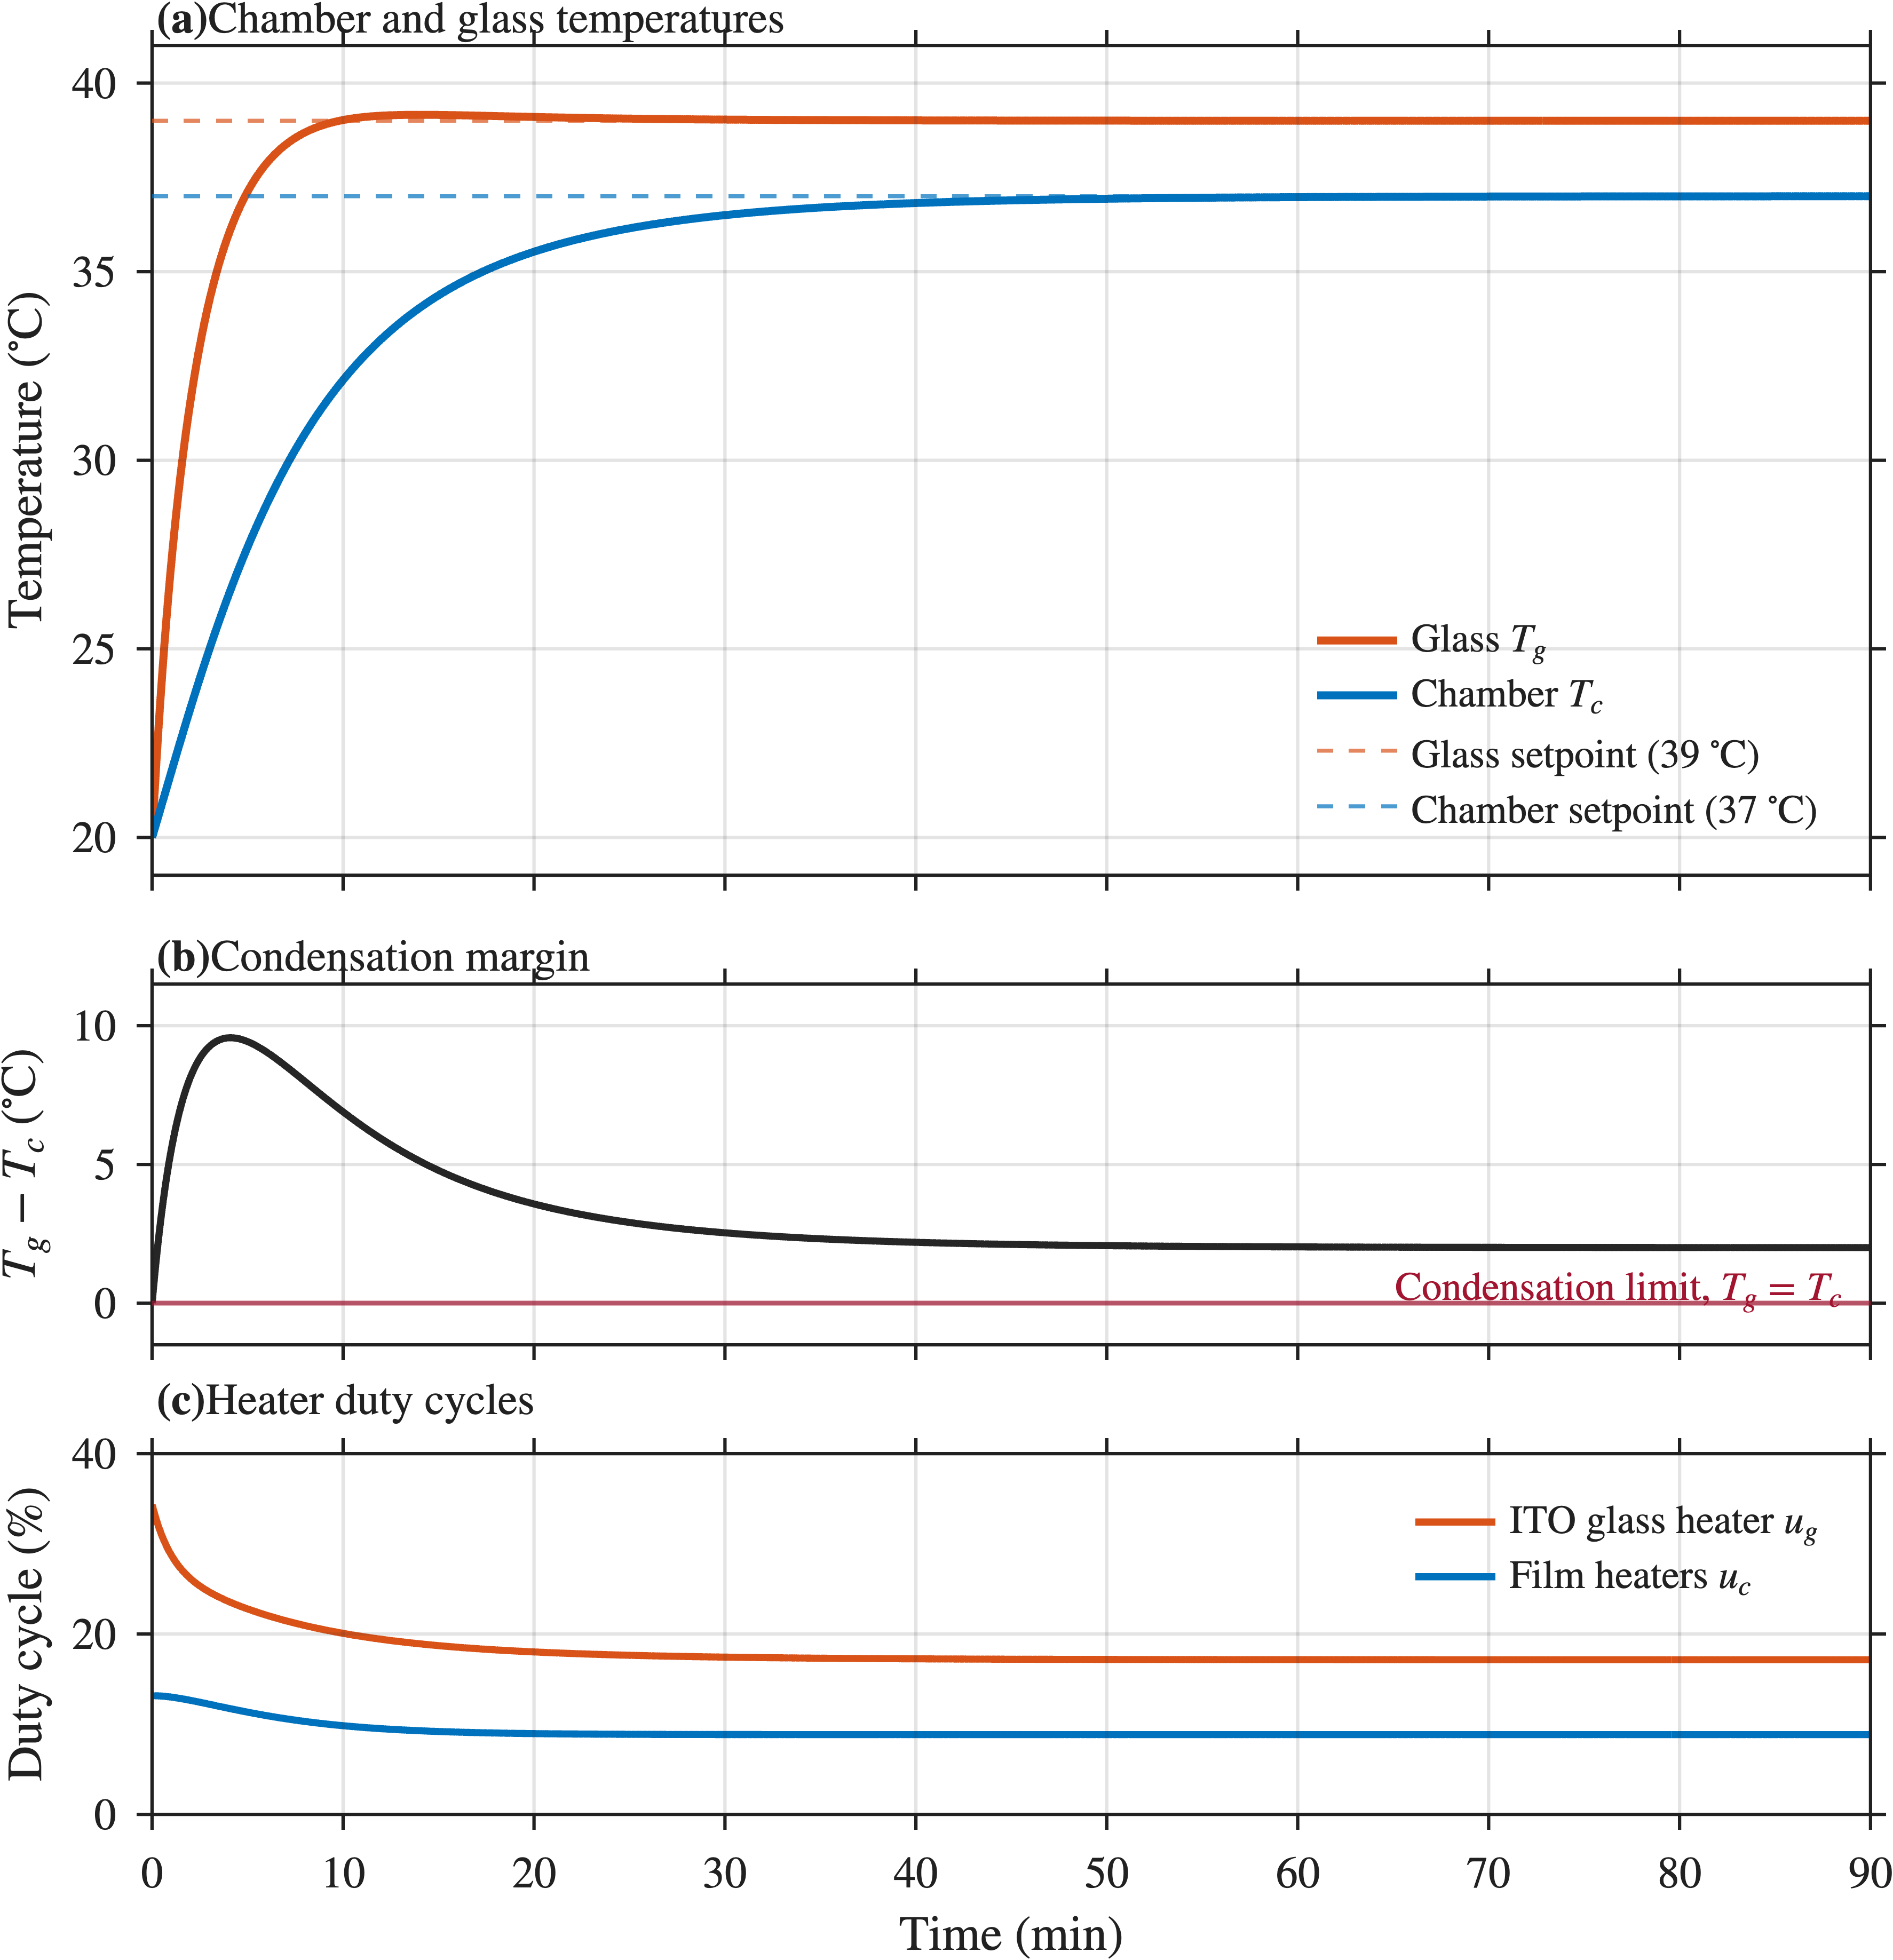
\includegraphics[width=0.78\textwidth,height=0.38\textheight,keepaspectratio]{figs/Control Simulation Figures/fig_T2_coupled_warmup.png}
    \caption[Coupled warm-up of the chamber and glass]{\textbf{Coupled warm-up of the chamber and glass.} (a) Temperatures and setpoints. (b) Glass-to-chamber margin, which must stay above zero. (c) Heater duty cycles.}
    \label{fig_T2_coupled_warmup}
\end{figure}

The coupled loops were simulated in Simulink (Figure~\ref{fig_T1_simulink}) and in MATLAB, starting at 20\,\textdegree{}C with a 20\,\textdegree{}C ambient. Figure~\ref{fig_T2_coupled_warmup} shows the warm-up: the glass reaches 39\,\textdegree{}C in about 8\,min and the chamber reaches 37\,\textdegree{}C in about 40\,min with no overshoot. The glass overshoots by 0.16\,\textdegree{}C as the warming chamber pushes it up, which is harmless, and it stays at least 2\,\textdegree{}C above the chamber throughout. Setpoint weighting is what keeps that warm-up clean: a standard PI ($b = 1$) overshoots by 0.48\,\textdegree{}C in the chamber and 0.43\,\textdegree{}C on the glass, because the warm glass adds slow extra heat to the chamber after the fast setpoint response has already arrived, which the linear design does not predict. With $b = 0.5$ the chamber overshoot is removed at the cost of a slower warm-up (Figure~\ref{fig_T4_setpoint_weighting}).

The room cooling from 20 to 16\,\textdegree{}C as a sudden step causes a dip of 0.73\,\textdegree{}C in the chamber, recovered within about an hour, which is outside R1, while the same change as a realistic two hour ramp causes only 0.12\,\textdegree{}C and stays well inside it (Figure~\ref{fig_T5_ambient_disturbances}). A 4\,\textdegree{}C step is a worst case rather than a laboratory condition, so the ramp is the case the requirement is judged on. With the gains fixed, the chamber loop stays stable for a capacitance from 110 to 250\,J/K and $\pm30$\% heater power, with a worst case overshoot of 0.2\,\textdegree{}C (Figure~\ref{fig_T6_robustness}), and both loops have a phase margin of 90$^\circ$ that a 30\,s delay reduces to no less than 61$^\circ$ (Figure~\ref{fig_T8_bode_nichols}). Running at $T_s = 1$\,s moves the discrete closed loop poles by less than 0.0001 from the continuous ones (Figure~\ref{fig_T9_discrete_vs_continuous}).

\subsection{CO\textsubscript{2} Control}
\label{subsec:co2-control}


The solenoid is driven by time-proportioning on a $T_s = 15$\,s period, and the sensor datasheet quotes a response of under 30\,s without naming the percentage it refers to \citep{gss_explorir_m}. Read as $T_{90}$, a first order lag has $\tau_s = T_{90}/\ln 10 \approx 13$\,s. Half the control period and half the averaging window add to this, so about 25\,s passes before the loop sees a change, and mixing in the chamber adds more. Reading the 30\,s as $T_{63}$ instead would put $\tau_s$ at 30\,s, which costs about five degrees of phase at the crossover and changes nothing in the design. $\lambda = 200$\,s stays well clear of either while still reaching 5\,\% in about 10 minutes. Setpoint weighting is not used: the CO\textsubscript{2} time constant is over eight times $\lambda$, so with $b < 1$ the slow plant mode in Equation~\ref{eq:setpoint-weighting} would stretch the fill to over an hour.

\begin{figure}[htbp]
    \centering
    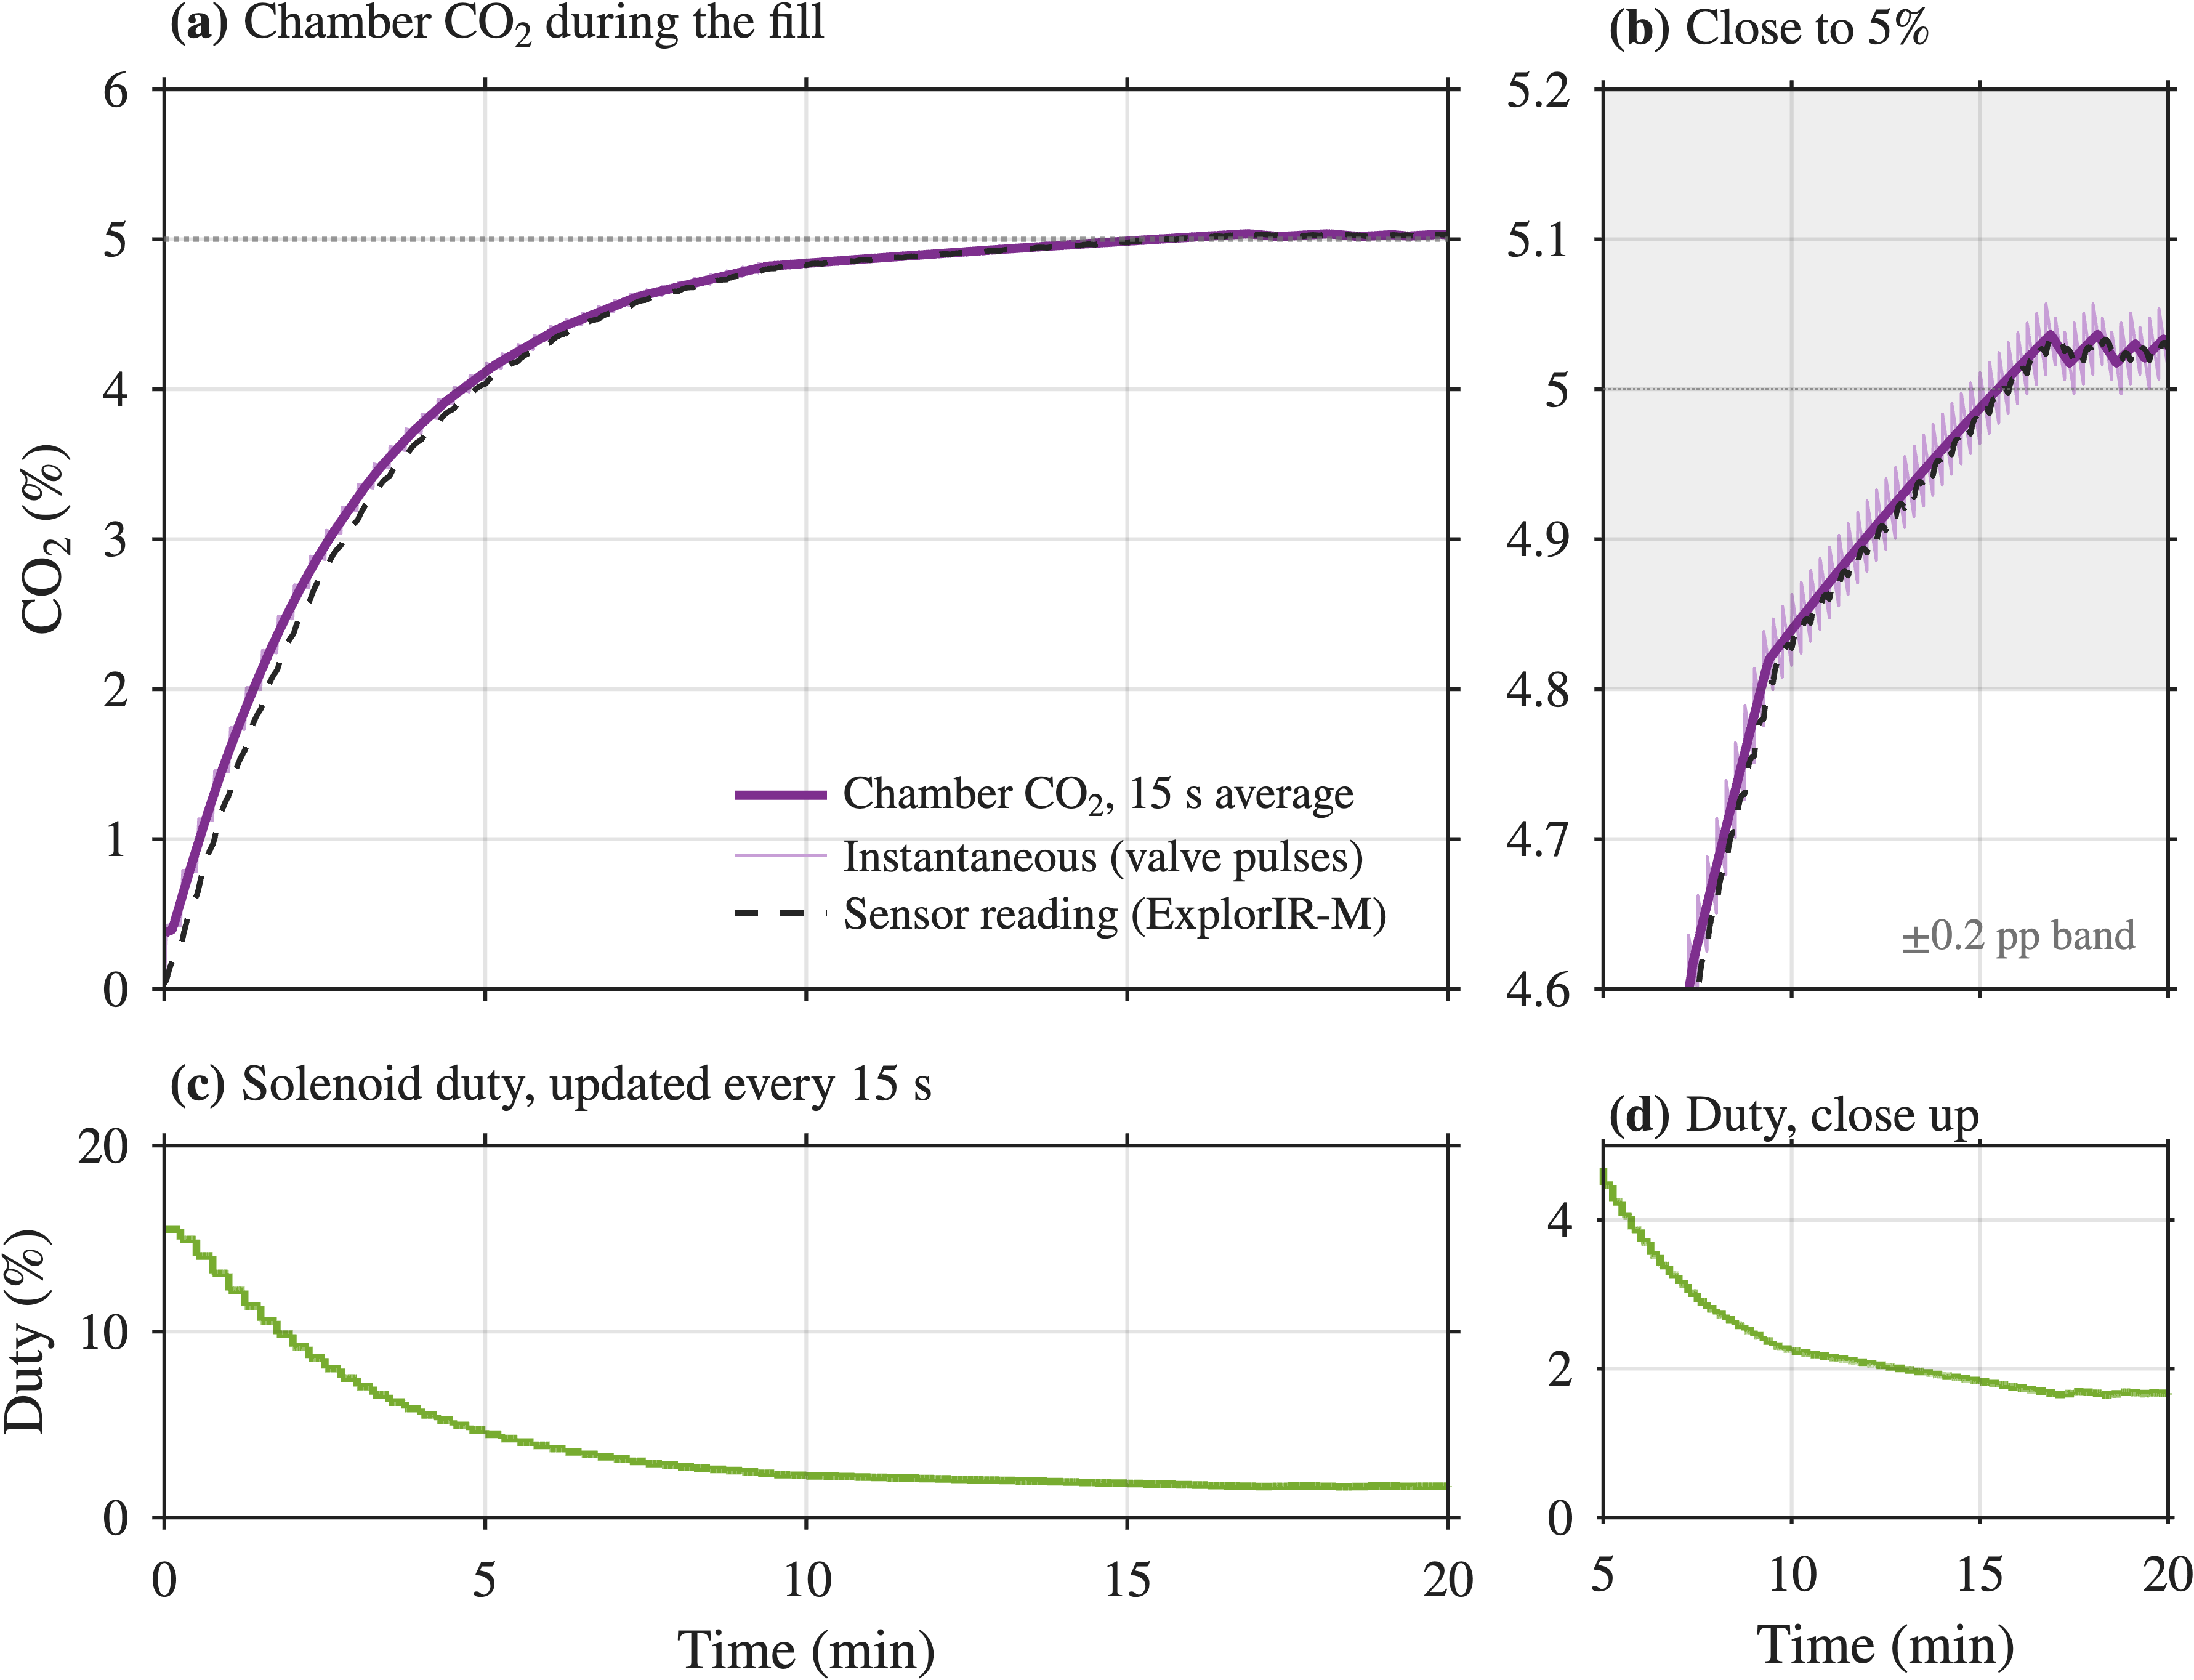
\includegraphics[width=0.78\textwidth,height=0.38\textheight,keepaspectratio]{figs/Control Simulation Figures/fig_C2_fill.png}
    \caption[CO\textsubscript{2} fill from room air]{\textbf{CO\textsubscript{2} fill from room air.} (a, b) Concentration and sensor reading, with a $\pm$0.2\,pp band shaded in (b), tighter than the $\pm$0.3\,pp of R4. (c, d) Solenoid duty.}
    \label{fig_C2_fill}
\end{figure}

Because the nonlinearity is mild, filling from room air is handled by the same PI as a large setpoint step. Holding the valve fully open until the sensor reads close to 5\% was rejected: the chamber fills in about 30\,s, faster than the sensor responds, and in simulation this overshot to 7.2\%, which took about 45\,min to leak away (Figure~\ref{fig_C3_fill_strategies}). A second problem appears after the lid is opened, where the integral builds up during the recovery and pushes the concentration past 5\%. The integral is therefore frozen whenever the error exceeds 0.5\,pp, but only once the chamber has first reached 5\%, by which point it already holds the steady duty for the real chamber.

The loop was built in Simulink with the linear model (Figure~\ref{fig_C1_simulink}) and the test cases were run in MATLAB with the nonlinear balance of Equation~\ref{eq:co2-balance}, the sensor lag and the pulsed valve. Figure~\ref{fig_C2_fill} shows the fill from room air: 5\% is reached in about 10\,min with less than 0.1\,pp of overshoot, and the duty settles at the predicted 1.7\%, as one short valve opening in each 15\,s window (Figure~\ref{fig_C6_valve_pulses}). After a full loss to 1\% through a lid opening, the plain PI overshoots by about 0.3\,pp for over 30\,min, while with the integrator freeze the overshoot is below 0.1\,pp and the chamber recovers in about 10\,min (Figure~\ref{fig_C4_lid_openings}). The loop remains stable with the leak halved or tripled and the flow halved or doubled (Figure~\ref{fig_C5_robustness}), and keeps a phase margin of 83$^\circ$ with the sensor lag and sampling included (Figure~\ref{fig_C7_bode}).

All values in this chapter are estimates. Each loop is re-identified from step tests on the built chamber in Chapter~\ref{ch:thermalID}, and the gains are recalculated from Equation~\ref{eq:lambda-gains} with $\lambda$ replaced by $\lambda + \theta$, where $\theta$ is any measured delay. The controller structure and the simulation models stay the same.